\documentclass[12pt]{article}
\usepackage{SteveStyle}
\usepackage{mathtools} % for lightning bolt
\newcommand{\ntap}{n_{tap}}
\newcommand{\nchan}{n_{chan}}
\newcommand{\lblock}{l_{block}}

% \usepackage{hyperref}
\usepackage[colorlinks = true,
            linkcolor = blue,
            urlcolor  = blue,
            citecolor = blue,
            anchorcolor = blue]{hyperref}

\begin{document}

\title{Inverting the Polyphase Filter Bank draft}
\author{Stephen Fay, Jon Sievers}
% \date{June 1st 2021}
\maketitle

\tableofcontents

\begin{abstract}
    The polyphase filter bank (PFB) is a widely used digital signal processing tool used for channelizing input from radio telescopes. Quantization of the channelized signal leads to blow ups in error. We present a practical method for inverting the PFB with minimal quantization-induced error that requires as little as 3\% extra bandwidth.
\end{abstract}



\section{Introduction}


Polyphase filter banks (PFBs) are widely used in digital signal processing to provide flat response within frequency channels and excellent rejection of out-of-band signals. Several current and upcoming radio arrays (CHIME, HIRAX, ALBATROS, CHORD) will record baseband data that has gone through a PFB, which will later be post-processed. A regular feature of the post-processing is to rechannelize data since finer frequency resolution can be provided by the original (usually FPGA-based) PFBs is often required. The natural way to do this is to invert the PFB to return to the original electric field samples. \\ %Unfortunately, quantization effects generally will induce spurious noise into the inverse-PFB, so in practice a carefully constructed pseudo-inverse will be preferred. To see how such a pseudo-inverse would be made, we first show how the forward PFB is constructed using the notation of linear algebra. \\ 

% The forward PFB is essentially a down-sampled spectrogram where the overlap between DFT'd segments (aka `sliding windows') exactly compensates for the down sampling so that the same quantity of signal data go out than come in. \\ 

Quantizing the output of a PFB leads to channel-specific loss of information, this causes spurious time-localized blow ups the inverted PFB error (cite paper, JS's write-up). By saving a small amount of terms of the raw input we are able to re-construct a pretty accurate inverse. This is accomplished by casting the problem as a chi-squared minimization. We use the conjugate gradient method to solve it efficiently. \\ 

In section \ref{sec:forward pfb} we present the forward PFB mathematically, in the language of linear algebra. In section \ref{sec:inverse pfb prior} we cover a first attempt at inverting the PFB and take a look at the errors induced by quantization. We also briefly discuss a failed attempt at modifying the sinc-hanning window to rid the virgin PFB of blow-ups in error. In section \ref{sec:conjugate gradient ipfb} we demonstrate how a signal can be reconstructed from a minimal amount of data. 

\section{Forward PFB}\label{sec:forward pfb}

% lets use ntap, nchan and lblock for the paper, and lets use m, n, b for the 'pedagogical writeup'
\textit{For ease of notation $n \equiv \nchan$ is the number of output channels of the PFB, $m \equiv \ntap$ is the number of taps, $b \equiv \lblock = 2(n-1)$ is the length of a segment (or `block'). Typical numbers are $n=1025$, $m=4$ and $b=2048$. } \\

The goal of the PFB is to split a stream of electric field data up into frequency channels, where the response inside a channel is flat, and the response outside the channel dies as quickly as possible. \\

The ideal thing to do would be to Fourier transform the electric field and average over neighbouring frequency channels (average over $\ntap$ channels). This is equivalent to convolving the output of the DFT'd signal with a boxcar then down-sampling by a factor of $\ntap$. By the discrete convolution theorem, this is equivalent to fourier transforming the pointwise multiplication of the original signal with the DFT of the boxcar, and down-sampling that. Down-sampling a fourier transform (by a factor of $\ntap$) is the same as fourier-transforming a shorter signal, each term of this shorter signal is just the sum of $\ntap$ terms of our original signal. This way the we reverse the order of operations so as to down-sample before Fourier transforming. \\

% alternative wording of same paragraph
The goal of the PFB is to split a stream of electric field data up into frequency channels, where the response inside a channel is flat, and the response outside the channel dies as quickly as possible. To accomplish this we can fourier transform (DFT) a segment of our E field signal and then sum over each frequency bin (i.e. each channel.) Which is equivalent to sampling from the convolution of the FT with a boxcar. The convolution theorem states that the iDFT of a convolution of two sequences is equal to the pointwise multiplication of the iDFT of the sequences. The iDFT of a boxcar is the sinc function, the iDFT of the DFT of the segment. Hence we can reverse the order of operations: we multiply our E field segment with a sinc window before applying a DFT the result, and then downsample. And here's where we make the observation that a down sampled DFT, decimated by a factor of $\ntap$ is the same as the DFT of the sum of a stack of $\ntap$ pieces of the segment. \\

% this line elaborates the above
In case the above paragraph wasn't clear to the reader we re-word it precisely in the language of linear algebra: The core computation of the PFB is the successive application of three matrices \tbf{FSW}: \tbf{F} is a real DFT; \tbf{S} is a horizontal stack of $\ntap$ square $b \times b$ identity matrices -it chops up a segment of raw signal into $\ntap$ pieces and sums them with each other; and \tbf{W} is a square diagonal sinc window matrix, it multiplies the raw input block by a sinc window (in practice we use a sinc-hanning window to further reduce the sidelobes.) \\

\begin{equation}\label{eq:W matrix}W : [g_1,\cdots,g_{bm}] \mapsto [g_1\cdot w_1,\cdots,g_{bm}\cdot w_{bm}]\end{equation}

The forward PFB takes a signal (a \textit{real} 1D array) of length $kbm$, where $k$ is some natural number (lets say $k=50$, in reality $k$ will be on the order of $10^5++$). It eats a $b\cdot m$ long segment and spits out $n$ \textit{complex} values, one for each frequency channel. Then it slides along the input signal by $b$ and repeats. \\

Ignoring the FFT component, i.e. considering only the action of $SW$ on the time-stream. Our forward PFB can be represented in the following way 

$$
g(t) = [g_1,\cdots,g_{kbm}]
    \begin{aligned}
        &\longrightarrow [g_{1},\cdots,g_{bm}] && \stackrel{W}{\longrightarrow} [g_1w_1,\cdots,g_{b m}w_{bm}] \\
        &\longrightarrow [g_{b+1},\cdots,g_{b+bm}] && \stackrel{W}{\longrightarrow} [g_{b+1}w_1,\cdots,g_{bm+b}w_{bm}] \\
        &\,\,\cdots\cdots\cdots\cdots\cdots\cdots\cdots && \,\,\cdots\cdots\cdots\cdots\cdots\cdots\cdots\cdots \\
        &\longrightarrow [g_{kbm-bm},\cdots,g_{kbm}] && \stackrel{W}{\longrightarrow} [g_{kbm - bm}w_1,\cdots,g_{k b m}w_{bm}] 
    \end{aligned}
$$

$$
\begin{aligned}
    &\stackrel{S}{\longrightarrow}\\
    &\stackrel{S}{\longrightarrow} \\
    &\,\,\cdots \\ 
    &\stackrel{S}{\longrightarrow}
\end{aligned}
\quad\sum_{j=0}^{ m-1}
    \begin{bmatrix}
        g_{jb+1}w_{jb+1} \,, & \cdots\,, & g_{b(j + m)}w_{b(j+m)}\\
        g_{b(j+1)+1}w_{jb+1} \,,& \cdots\,, & g_{b(j+m+1)}w_{b(j+m)}\\
        g_{jb+2b+1}w_{jb+1} \,,& \cdots\,, & g_{b(j+m+2)}w_{b(j+m)}\\
        \cdots&\cdots&\cdots\\
        g_{b(km-1)+1}w_{jb+1} \,,&\cdots\,, & g_{kbm}w_{b(j+m)}
    \end{bmatrix}
$$

For clarity we write this block with $m = 4$ and $b = 16$ and $k=50$

\begin{equation}\label{eq:matrix output SW}
\begin{bmatrix}
g_1w_1+g_{17}w_{17}+g_{33}w_{33}+g_{49}w_{49} & \cdots & g_{16}w_{16}+g_{32}w_{32}+g_{48}w_{48}+g_{64}w_{64}\\
g_{17}w_1+g_{33}w_{17}+g_{49}w_{33}+g_{65}w_{49} & \cdots & g_{32}w_{16}+g_{48}w_{32}+g_{64}w_{48}+g_{80}w_{64}\\
\cdots & \cdots & \cdots \\
g_{3137}w_{1}+g_{3153}w_{17}+g_{3169}w_{33}+g_{3185}w_{49} & \cdots & g_{3152}w_{16}+g_{3168}w_{32}+g_{3184}w_{48}+g_{3200}w_{64}
\end{bmatrix}
\end{equation}

Now the fourier transform. In some implementations (such as \href{https://github.com/jrs65/pfb-inverse}{Richard Shaw's python implementation} of the Chime PFB) the $S$ matrix is not applied, instead $FW$ is down-sampled by a factor of $m$. \\ 

In the end the result is the same. Let $\downarrow$ represent down-sampling by a factor of $\ntap\equiv m$, and let $F_b$ be the $b\times b$ DFT matrix, then $\downarrow F_{bm}W = F_{b}SW$. To make this evident first observe that they are both $bm \times b$ matrices, and that their action on an arbitrary vector $v$ is the same

$$\begin{aligned}\left[\downarrow FW v\right]_k &= \sum_{j=0}^{bm-1}\exp{-2\pi i\frac{mk j}{mb}}w_{j} v_j\\ 
&= \sum_{j=0}^{b-1}\exp{-2\pi i\frac{kj}{b}}\left(\sum_{r=0}^{m-1}w_{br + j}v_{br+j}\right)\\ &= \left[ FSW v \right]_k \end{aligned}$$

Where $w_j$ is the $jj$'th entry of $W$, we use a single subscript because $W$ is diagonal. There is a funny thing going on with the indexing when we use \code{rfft}, but everything works out. Applying the real fast fourier transform to an array of even length $bm$ will return an array of length $bm/2+1$. In the first case when we down-sample we will end up with $b/2 + 1 \,\,(\equiv n)$ samples, when we apply $FSW$ we end up with the \code{rfft()} swallowing $SW v$ - which has length $bm/m = b$, thus the output also has $n$ output channels. It is left as an exercise to show that these are indeed equivalent. \\

If we flatten the output of the PFB by concatenating each row, the output is practically the same length as the input time-stream (it's actually $(\ntap-1)\cdot\lblock$ shorter, but we can ignore that given that the input is very long). If we let $m=4$, then \tbf{FSW} is the discrete fourier transform of a stack of four diagonal square matrices $SW = [D_1,D_2,D_3,D_4]$. So we can represent the (row-wise) inverse fourier transformed PFB as a large almost-square matrix

\begin{equation}\label{eq:pfb matrix}
\begin{bmatrix}
    D_1 & D_2 & D_3 & D_4 & &&& \\
    & D_1 & D_2 & D_3 & D_4 & && \\ 
    && D_1 & D_2 & D_3 & D_4 & & \\ 
    &&& \ddots & \ddots & \ddots & \ddots & \\
    &&&&  D_1 & D_2 & D_3 & D_4
\end{bmatrix}
\end{equation}

% It is handy to introduce a matrix very much like \eqref{eq:pfb matrix} but that is actually square, by adding $m-1$ rows.

% \begin{equation}\label{eq:pfb matrix square}
% \begin{bmatrix}
%     D_1 & D_2 & D_3 & D_4 & &&& \\
%     & D_1 & D_2 & D_3 & D_4 & && \\ 
%     && D_1 & D_2 & D_3 & D_4 & & \\ 
%     &&& \ddots & \ddots & \ddots & \ddots & \\
%     &&&&  D_1 & D_2 & D_3 & D_4 \\ 
%     D_4 &&&&& D_1 & D_2 & D_3 \\ 
%     D_3 & D_4 &&&&& D_1 & D_2 \\ 
%     D_2 & D_3 & D_4 &&&&& D_1
% \end{bmatrix}
% \end{equation}



\section{Inverting the PFB, a first attempt}\label{sec:inverse pfb prior}

\textit{Reminder: for ease of notation we use $n=\nchan$ is the number of output channels of the PFB, $m=\ntap$ is the number of taps, $\lblock = 2(n-1) = b$ is the length of a segment.} \\

Inverting the PFB amounts to retrieving the windowed time-stream points $g_i$ from the above block matrix \eqref{eq:matrix output SW}. The first column $v$ of this matrix is \eqref{eq:column vector SW timestream} 

\begin{equation}\label{eq:column vector SW timestream}
h^{(1)} = 
    \begin{bmatrix}
        g_1w_1+g_{17}w_{17}+g_{33}w_{33}+g_{49}w_{49}\\
        g_{17}w_1+g_{33}w_{17}+g_{49}w_{33}+g_{65}w_{49}\\
        \cdots\\
        g_{3121}w_1+g_{3137}w_{17}+g_{3153}w_{33}+g_{3169}w_{49}\\
        g_{3137}w_1+g_{3153}w_{17}+g_{3169}w_{33}+g_{3185}w_{49}
    \end{bmatrix}
    \longleftrightarrow
    \begin{bmatrix}
        \sum_{j=0}^{m-1} g_{bj + 1}w_{bj + 1}\\
        \sum_{j=0}^{m-1} g_{bj + b + 1}w_{bj + 1}\\
        \cdots \\
        \sum_{j=0}^{m-1} g_{bmk-b(m-j)}w_{bj + 1}
    \end{bmatrix}
\end{equation}
\vspace{0.25cm}

Technically speaking this problem is insoluble. To solve it practically we introduce circulant boundary conditions by appending the first $m-1$ terms of $h_1$ to it's tail. \\

Notice that $v$ this is equivalent to the convolution of

$$\widetilde g^{(1)}:= [g_1,g_{17},g_{33},\cdots,g_{3121},g_{3137},g_1,g_{17},g_{33}]$$

with a flipped, zero padded and rolled `chunk' of window 

$$\widetilde w^{(1)} = [w_1,0,0,\cdots,0,0,w_{49},w_{33},w_{17}]$$ 

Indeed

$$h^{(1)} := \widetilde w^{(1)}\ast \widetilde g^{(1)} = [g_1w_1+g_{17}w_{17}+g_{33}w_{33}+g_{49}w_{49} \,,\, g_{17}w_1+g_{33}w_{17}+g_{49}w_{33}+g_{65}w_{49}\,,\,\text{etc.}]$$

\textit{Note on the notation:} $\widetilde g^{(r)}[t]$ is the $t$'th element of the $r$'th recovered time-stream $[g_r,g_{r+17},\cdots]$. The integer $r$ denotes the channel index. We use $r=1$ so that the notation doesn't become heavy-handed, but this method works for every channel. \\   

Invoking the discrete convolution theorem (see appendix section \ref{sec:discrete conv thm}) we see that

$$\mathcal F[\widetilde w \ast \widetilde g](\xi) \equiv \mathcal F [h](\xi) = \widehat h(\xi) = \widehat w(\xi)\cdot \widehat g(\xi)$$

solving for $\widetilde g = \mathcal F^{-1} G$, we recover the original time-stream.

\begin{equation}\label{eq:reconstructed signal}
\widetilde g^{(1)}[t] = \mathcal F^{-1}\Big[ \widehat h^{(1)}(\xi) / \widehat w^{(1)}(\xi)\Big][t] = \mathcal F^{-1} \Big[\mathcal F[h^{(1)}](\xi) / \mathcal F[\widetilde w^{(1)}](\xi) \Big] = [g_1,g_{17},g_{33},\cdots]
\end{equation}


\subsection{Quantisation effects}

This solution works well if our data is clean and precise. But in practice the vectors $h^{(i)}$ are quantized. Which is effectively the same as introducing Gaussian random noise to $\widehat h(\xi)$. Problems arise when $\widehat w^{(i)}(\xi) = \mathcal F [\widetilde w^{(i)}](\xi)$ approaches zero. i.e. when the fourier transform of $[w_1,w_{17},w_{33},w_{49},0,0,0,\cdots]$ is close to zero (the blue parts in figure \ref{fig:eigenvalues sinc hanning ntap=4}) 

\begin{figure}[H]
    \centering
    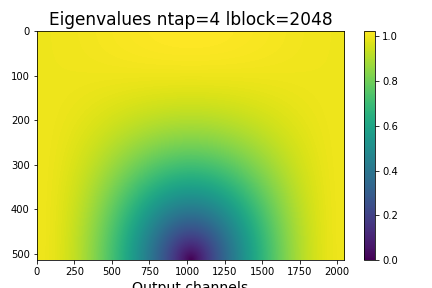
\includegraphics[width=0.49\linewidth]{figures/eigenvalues_ntap/eigenvalues_ntap_4_lblock_2048.png}
    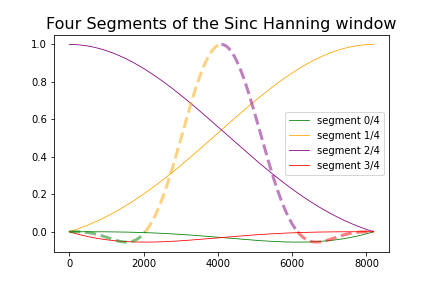
\includegraphics[width=0.49\linewidth]{figures/four_segments_of_sinc_hanning.png}
    \caption{Left Hand Side: On the $x$ axis we have the \code{irfft} (inverse real discrete fourier transform) of the 1025 output channels of the PFB (rem $(1025-1)\times 2 = 2048$.) The y axis are the absolute values of the fourier transforms of the zero padded sinc-hanning window chunks: $\text{DFT} [w_x,w_{x+2048},w_{x+2\cdot 2048},w_{x+3\cdot 2048},0,\cdots,0]$. The middle columns have the unfortunate property that it's four terms are symmetric $w_x \approx w_{x+3\cdot 2048}$ and $w_{x+2048}\approx w_{x+2\cdot 2048}$ the fourier transform contains zeros.\\
    Right Hand Side: The sinc-hanning window and it's four segments. One column of the LHS is generated by concatenating four terms -one from each segment of the corresponding vertical slice of the RHS image- with many zeros ($\approx 1000$), applying the \code{rfft} and taking the modulus of each term in the resulting vector.}
    \label{fig:eigenvalues sinc hanning ntap=4}
\end{figure}

Lets examine more closely how the mean squared error (MSE) from quantization carries forward. The effect of quantizing a signal $h[n]$ is for our purposes identical to adding a random variable $x[n]$ which is a uniform probability distribution on $(-\Delta/2,\Delta/2]$. Where $\Delta$ is the quantization interval. It is easy to see that the MSE induced from the quantization is $\Delta^2/12$ \eqref{eq:MSE quantization}

\begin{equation}\label{eq:MSE quantization}
    \text{MSE} = \frac{1}{\Delta}\int_{-\Delta/2}^{\Delta/2} dx\, x^2 = \Delta^2/12
\end{equation}

An important fact that simplifies our lives is that the expected value of the MSE of the discrete fourier transform of a quantized signal is identical to that of the quantized signal, i.e.

\begin{equation}\label{eq:MSE invariant under DFT}
\langle |x[n]^2| \rangle = \langle |\widehat x[\xi]|^2\rangle = \left\langle \left| \frac{1}{\sqrt N}\sum_{n=1}^N x[n] e^{-2\pi i \xi n/N}\right|^2 \right\rangle
\end{equation}
since

\begin{equation}
\begin{split}
    \langle |\widehat x[\xi]|^2\rangle 
    & = \left\langle \left| \frac{1}{\sqrt N}\sum_{n=1}^N x[n] e^{-2\pi i \xi n/N}\right|^2 \right\rangle \\
    &= \left\langle \frac{1}{N}\sum_n x[n]x[n]^\ast + \frac{1}{N} \sum_{n > m}\big(x[n]x[m]^\ast + x[n]^\ast x[m]\big)\right\rangle \\
    &= \langle \langle |x[n]|^2\rangle \rangle = \langle |x[n]|^2 \rangle
\end{split}
\end{equation}

The same is true for the inverse DFT. Letting $\sigma^2 = \Delta^2/12$ denote the MSE of our output and channalized signal $h$ (output of forward pfb) and using equation \eqref{eq:reconstructed signal} we find the MSE of the reconstructed signal $\widetilde g$ (output of the inverse pfb). 

\begin{equation}\label{eq:R factor}
\begin{split}
    \text{MSE}(\widetilde g^{(n)}[t]) &= \left\langle \left| \mathcal F^{-1} [\widehat x(\xi)/\widehat w^{(n)}(\xi)] \right|^2 \right\rangle \\
    &= \left\langle \frac{1}{k}\sum_{\xi=1}^k |\widehat x(\xi)/ \widehat w^{(n)}(\xi)|^2 \right\rangle \\
    &= \langle \widehat x^2 \rangle \cdot \frac{1}{k}\sum_{\xi=1}^k  \frac{1}{|\widehat w^{(n)}(\xi)|^2} \\
    &= \sigma^2 \cdot R[n]^2 \cdot 12 \qqquad\text{where}\quad R[n]:= \sqrt{ \frac{1}{12\cdot k}\sum_{\xi=1}^k \frac{1}{|\widehat w^{(n)}(\xi)|^2} } \\
    \RA\text{RMSE}(\widetilde g^{(n)}[t]) &= \Delta \cdot R[n] 
\end{split}
\end{equation}

Where $\widehat x$ is the same uniform random variable on $[-\Delta/2,\Delta/2)$ as before. See figure \ref{fig:quantization RMSE} \\ 

When $\widehat w^{(n)}[\xi]$ has near-zero terms $R[n]$ becomes very large and so too does the the error. 

\begin{figure}[H]
    \centering
    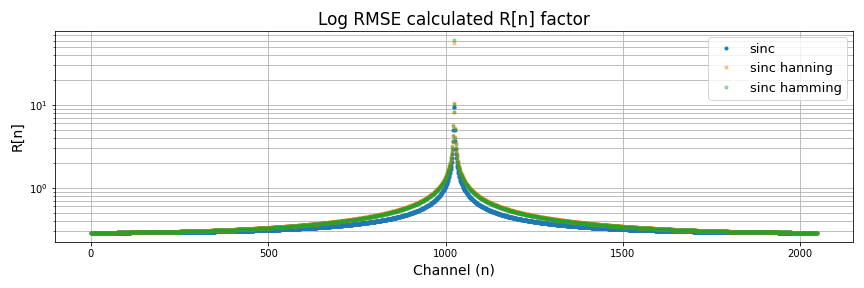
\includegraphics[width=\linewidth]{figures/rmse/Log_RMSE_calculated.png}
    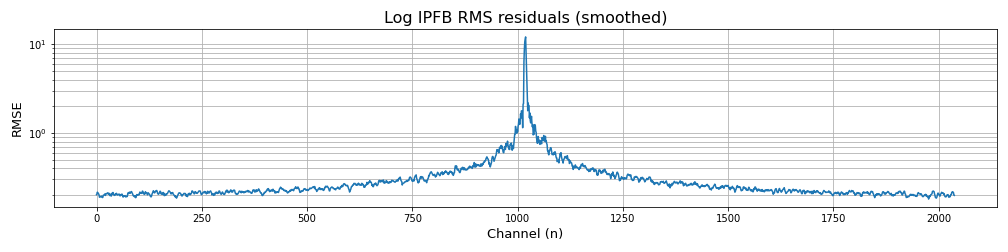
\includegraphics[width=\linewidth]{figures/rmse/Log_virgin_IPFB_RMS_residuals_0.png}
    
    \caption{Top: $R[n]$ as described above \eqref{eq:R factor}, calculated for three windows. Bottom: the RMSE on data points from each channel for the virgin IPFB with quantization interval $\Delta=0.5$, obtained via simulation. The fact that the two plots are the same up to a factor of $\Delta$ confirms our above derivation of $R[n]$. }
    \label{fig:quantization RMSE}
\end{figure}

\subsection{Why do some eigenvalues go to zero?}

Let $\omega[n]$ be a sinc hanning window of length $4b$ indexed from $-2b$ to $2b$  (or indeed a sinc / sinc-hamming). These windows are symmetric $\omega[n] = \omega[-n]$. Now consider the DFT of a real valued array $\big[\omega[k-2b],\omega[k-b],\omega[k],\omega[k+b],0,0,0,0,0,\cdots,0\big]$, (which corresponds to the $k$'th column of eigenvalues from \ref{fig:eigenvalues sinc hanning ntap=4}.)

$$\mathcal F[\omega[k-2b],\omega[k-b],\omega[k],\omega[k+b],0,0,\cdots,0](k) = \omega[k-2b] + \omega[k-b] e^{-2\pi i \frac{k}{4b}} + \omega[k] e^{-2\pi i\frac{2k}{4b}} + \omega[k+b] e^{-2\pi i\frac{3k}{4b}}$$

The value of $k$ ranges from $1$ to $b$ (we can ignore $k>b/2$ because the signal is real, hence FFT symmetric). As we see from figure \ref{fig:eigenvalues sinc hanning ntap=4}, the values that are causing trouble by being small are the ones at the bottom, i.e. when $k=b/2$. These zeros correspond to symmetric w-chunks. By symmetry $\omega[b/2-2b]=\omega[b/2+b]$ and $\omega[b/2-b]=\omega[b/2]$, therefore the above sum is 

$$\omega[-3b/2] - \omega[-b/2] + \omega[b/2] - \omega[3b/2] = 0$$

\subsection{Can we modify the PFB window so as to avoid this?} 

\subsubsection{No: a mathematical argument.}

Assuming we don't break the symmetry of the sinc-hanning window $\omega$, i.e. that $\mathring \omega[n]=\mathring \omega[-n]$, where $\mathring \omega[n]$ is the modified window. Let $\phi[n] := \mathring\omega[n] - \omega[n]$. Then we require that the derivative $\phi'[n]$ be very steep in the middle of each of the four segments. If we consider that any eigenvalue who's absolute value is below $0.1$ is ``bad" (these are the eigenvalues responsible for magnifying the quantization error.) And we want there to be maximum 20 channels of bad eigenvalues (out of 2048 = 1\% of channels). Then we require \eqref{eq:condition 1}

\begin{equation}\label{eq:condition 1}10\cdot \phi'[k] > 0.1\end{equation} 

for $k=b/2$, $k=3b/2$. Now consider the fourier decomposition of $\phi(k)$

\begin{equation}\label{eq:fourier decomposition}
    \phi[k] \approx \sum_{s=1}^{8000} a_s \sin( s k/16000 )  
\end{equation}

We must keep the side-lobes below $10^{-7}$ so that there is minimal leaking. Each term $a_s$ contributes \textit{approximately} to a side-lobe as a delta function at the index of it's frequency. Therefore we require that $|a_s| < 10^{-7}$ for each $s$.

\begin{equation}
\begin{split}
    10^{-2} \stackrel{\eqref{eq:condition 1}}{<} |\phi'[k]| \leq 10^{-7} &\sum_{s=1}^{8000} \frac{s}{4\cdot 8000}\frac{2}{\pi}\\
    &\approx 10^{-7} \frac{8000^2}{4\cdot 8000}\frac{1}{\pi} \\
    &\approx 10^{-5} << 10^{-2}\qquad \text{\faBolt}
\end{split}
\end{equation}

In practice if you use this approach the side-lobes reach up to $10^{-4}$ before there is any noticeable improvement, and there isn't a way of making the zero eigenvalues disappear entirely without side-lobes which go the whole way up to $10^{-2}$. \\ 

\subsubsection{No: by trial and error.}
Here is what was tried:
\begin{itemize}
    \item Gradient descent to optimize the window (a vector of length $8192$) with a variety of loss functions that penalize low eigenvalues and large side-lobes. 
    \item GD in the fourier space of the window, with constraints on the fourier coefficients.
    \item Using GD to optimize a chebyshev (symmetric with constant term 1) filter.
    \item Modifying the eigenvalues themselves and re-constructing a window from them. This is a little bit non-trivial because the eigenvalue space has ($2\times$) more degrees of freedom than the window space (since they're complex.)
    \item Manual tinkering of the window: multiplying by polynomials, breaking the symmetry, applying hand crafted distortions to the domain before feeding it through a sinc-hanning function. (this was perhaps unsurprisingly the least successful approach)
\end{itemize}

For every loss function the gradient descent approach would preserve the symmetry of the window. Even when seeded with an asymmetric window (usually the starting point was the sinc-hanning window.) \\

See \code{gradient\_descent.py}, \code{gradient\_descent\_2.py} and \code{loss\_functions.py} in the \href{https://github.com/dcxSt/pfb-mod}{GitHub repository}, (other failed attempts are scattered in jupyter notebooks, not all pushed.)

\section{Correcting the inverse.}
\subsection{Weiner Filter}


\subsection{Constructing the most likely inverse-pfb with limited extra bandwidth (about 3\% extra).}\label{sec:conjugate gradient ipfb}

We examine the expected errors in each channel from the `virgin' IPFB described in the previous section. Using the notation of equation \eqref{eq:column vector SW timestream} 

$$h^{(r)} = [h^{(r)}[1],h^{(r)}[2],h^{(r)}[3],\cdots ,h^{(r)}[T]]$$

Quantizing $h^{(r)}[t]$ is equivalent to adding uniform noise with standard deviation to both real and imaginary components. The standard deviation for each component is $\sigma = \Delta/\sqrt{12}$ where $\Delta$ is the quantization interval. 

$$H^{(r)}[\xi] = \sum_{t=0}^T h^{(r)}[t]e^{-2\pi i t\xi /T}$$

The uncertainty on $h^{(r)}[t]$ induces an uncertainty in it's fourier transform $H^{(r)}[\xi]$. We write $H^{(r)}[\xi] + \hat x[\xi]$ where $\hat x[\xi]$ is a Gaussian random variable. 

$$\hat x[\xi] \sim \frac{1}{\sqrt{2\pi \sigma_0^2}} \exp\left( -\frac{1}{2}\frac{y^2}{\sigma_0^2} \right) \qquad\text{normal dist in $y$}\qquad \sigma_0 = \Delta/\sqrt{6}$$

As before the error carries forward

$$\langle g^{(r)}[t]\rangle = \left\langle \mathcal F^{-1} [(H^{(r)}[\xi] + \hat x(\xi)) / W^{(r)}(\xi)]  \right\rangle = \frac{1}{\sqrt T}\sum_\xi e^{2\pi i t\xi /T} H^{(r)}[\xi] / W^{(r)}[\xi] $$

\begin{equation}\label{eq:sigma 0}
\langle |g^{(r)}[t]|^2 \rangle - \langle g^{(r)}[t]\rangle^2 = \left\langle \mathcal \sum_{\xi =0}^{T-1} |\hat x[\xi]|^2 / |W^{(r)}[\xi]|^2 \right\rangle \frac{1}{T} = \sigma_0^2\left\langle\frac{1}{|W^{(r)}[t]|^2}\right\rangle =: \sigma_{(r)}^2
\end{equation}

We also have another $T$ equations, one for each frequency $\xi$

\begin{equation}\label{eq:coupled equations}
\frac{1}{\sqrt T}\sum_t e^{-2\pi i t\xi/T}g^{(r)}[t] = (H^{(r)}[\xi] + \hat x[\xi]) / W^{(r)}[\xi]
\end{equation}

\begin{equation}\label{eq:}
g^{(r)}[t] = \text{iDFT}\big[(H^{(r)}[\xi] + \hat x[\xi]) / W^{(r)}[\xi]\big] 
\end{equation}

Suppose that we know one fifth of the values of the discrete time series $g^{(r)}[t]$ (for instance that $g^{(r)}[0], g^{(r)}[4], g^{(r)}[9],...$ are known.) 

we cast it as a chi-squared problem \eqref{eq:chi-squared}. This we can minimize approximately and efficiently using conjugate gradient iterations. 

\begin{equation}\label{eq:chi-squared}
    \chi^2 = (d - Am)^T N^{-1} (d - Am) + (p - m)^T Q^{-1} (p - m)
\end{equation}

Where $d$ is the data (output of forward PFB), $m$ is the input to the PFB which we are solving for, $A$ is a matrix representing the forward PFB, $N^{-1}$ is a diagonal quantization noise matrix (with entries $1/\sigma^2$), $p$ is the prior (i.e. our preserved data-points) and $Q^{-1}$ is a diagonal matrix which represents the uncertainties in the prior.\\

\textit{Note on $Q^{-1}$:} for ease of notation we represent $p$ as the ground truth with a bit of quantization noise $\sigma_0$ (it's a factor of $\sqrt{2}$ smaller than $\sigma$ because the quantized terms are real with zero imaginary component), so that $Q^{-1}$ is filled on the diagonal with $1/\sigma_0^2$ at those places where we have preserved the term, and it's filled with $0$ in those places where we have not preserved the data point (most of them) representing infinite uncertainty. \\ 

\subsection{RMSE of simulated data with carefully selected 3\% extra.}

From the output of the PFB we select and preserve every $k$th term from the $q$ middle-most channels. The numbers $k$ and $q$ are constrained by how much extra space you have. If $k$ is large we can also afford to have a large $q$. We need $q$ to be thick enough to cover the worst channels. And we need $k$ to be small enough that it sufficiently fixes the contributions from each channel. \\

Figure \ref{fig:rmse 20 epochs comparison} shows the root mean squared errors for $k=6$ and $q$ such that exactly $3\%$ of the data is preserved. The results are very promising. 

\begin{figure}[H]
    \centering
    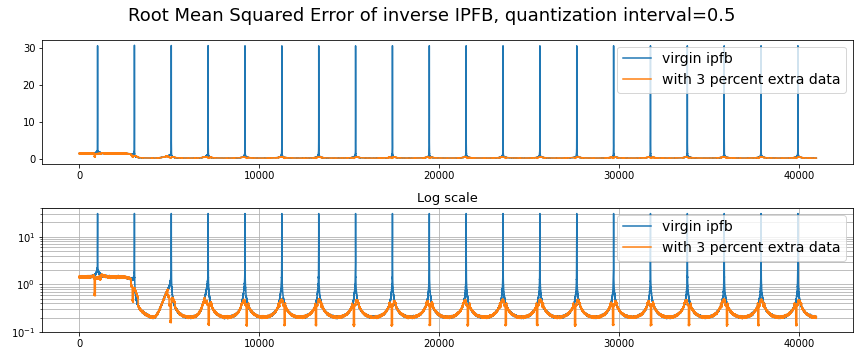
\includegraphics[width=\linewidth]{figures/rmse/RMSE_20_epochs_inverse_IPFB_vs_3perc_error_quantization_interval_0.5.png}
    \caption{Root mean squared error estimates calculated by simulating data, which is Gaussian Noise with sigma=1.0. The data is first passed through the forward IPFB. It then has both real and imaginary parts quantized with quantization interval $0.5$ i.e. a quantization noise sigma of $0.5/\sqrt{12}$ on each component. Then inverted with the method discussed in section \ref{sec:inverse pfb prior}, and improved upon with 3\% additional as described in this section (section \ref{sec:conjugate gradient ipfb}). Every 6'th data point is preserved from the middle $364$ channels (out of 2048).}
    \label{fig:rmse 20 epochs comparison}
\end{figure}

\subsubsection{Why does this work?}

One way to understand why this works so well is by thinking of a different solution (by constructing a pseudo-inverse PFB matrix from the set of linear equations + the data that we have) that works in theory but not in practice, and then understanding that our chi-squared method will perform better than this solution.\\

If we consider \eqref{eq:coupled equations} as a linear system of equations we can substitute the known values of $g^{(r)}$ and remove the need for equations containing small values of $W^{(r)}[\xi]$ (those error magnifying prone equations) effectively removing problematic eigenvalues as suggested in figure \ref{fig:eigenvalues}. \\ 

[change this paragraph, don't over-generalize, sometimes solving a system of equations w/ pseudo inverse is a good idea] In this case the pseudo inverse In practice solving a linear system of equations by computing a pseudo-inverse matrix is not a good idea. And our previous method of inverting the PFB is already quite good, except for these noise spikes. \\

Looking at our eigenvalues plot we can see that the most problematic $\widehat w^{(r)}$'s belong to the middle columns. These correspond to the mid frequency-range output channels. 

\begin{figure}[H]
    \centering
    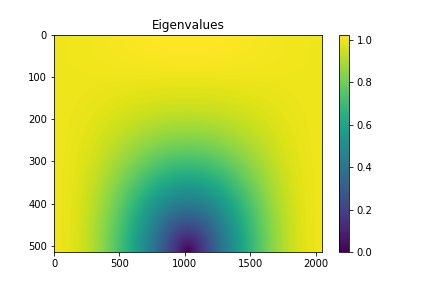
\includegraphics[width=0.32\linewidth]{figures/eigenvalues.png}
    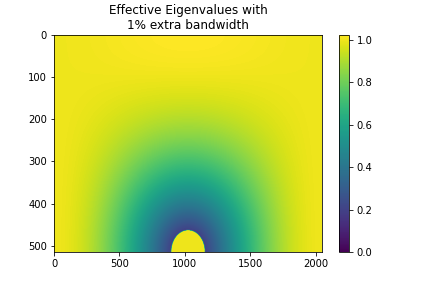
\includegraphics[width=0.32\linewidth]{figures/effective_eigenvalues_1perc_extra_bandwidth.png}
    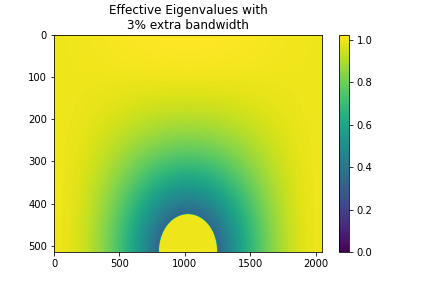
\includegraphics[width=0.32\linewidth]{figures/effective_eigenvalues_3perc_extra_bandwidth.png}
    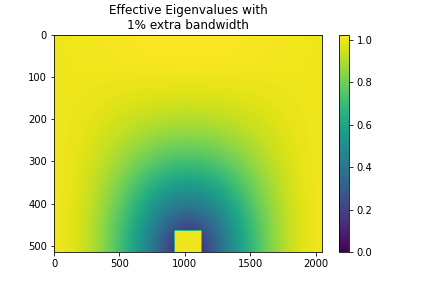
\includegraphics[width=0.32\linewidth]{figures/effective_eigenvalues_1perc_extra_bandwidth_implementable.png}
    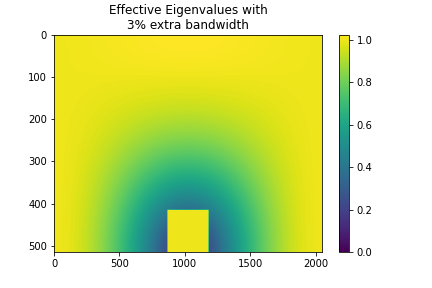
\includegraphics[width=0.32\linewidth]{figures/effective_eigenvalues_3perc_extra_bandwidth_implementable.png}
    \caption{Top from left to right: sinc-hamming window eigenvalues, eigenvalues with 1\% smallest blanked, eigenvalues with 3\% smallest blanked out.\\ 
    Bottom: Eigenvalues with 1\% blanked out in an implementable way. Eigenvalues with 3\% blanked out in an implementable way.\\ 
    We take our intuition that knowing one extra data-point is roughly equivalent to replacing the worst eigenvalue of it's corresponding column, from the inverse matrix method described in the appendix, because we expect chi-squared minimization to perform better than numerically computing a pseudo-inverse matrix.}
    \label{fig:eigenvalues}
\end{figure}




\subsection{Conjugate Gradient method for optimizing large quadratic systems of equations.}

[Little intro to conj grad with some pointers / citations to conj grad stuff. Show plot of how well it performs, and mention edge-effects.]

\begin{figure}[H]
    \centering
    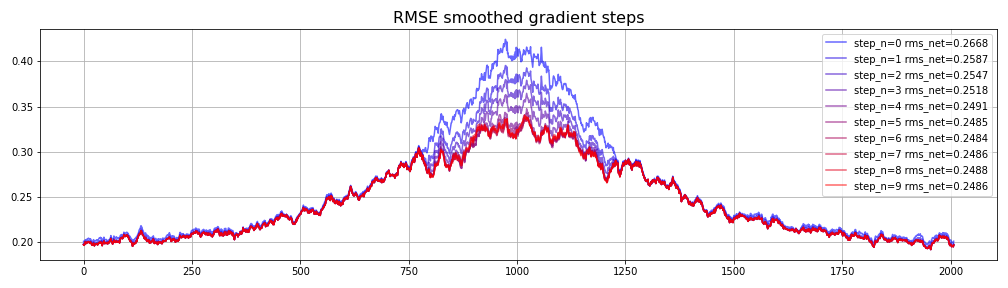
\includegraphics[width=\linewidth]{figures/rmse/RMSE_smoothed_gradient_steps_4.png}
    \caption{Estimated RMSE during conjugate gradient descent optimization of chi-squared. It converges very fast. The initial guess $x_0$ is a virgin IPFB with the badly behaved regions set to zero (hence the jump in RMSE.)}
    \label{fig:RMSE conj crad descent}
\end{figure}

Missing figures, put the Wiener filter thing in here. Noisy time-s


\section{Discussion}\label{sec:discussion} 


\section{Conclusion}\label{sec:conclusion} 


\section{Appendix}

\subsection{Discrete Fourier Transform}
The discrete fourier transform is a square symmetric matrix operator that acts on a complex or real vector space $\mathcal F : \C^N \to \C^N$. It's elements are $\mathcal F_{k,l} = e^{-2\pi i\frac{k\cdot l}{N}}/\sqrt N$. It looks like this

\begin{equation}\label{eq:fourier matrix}
\mathcal F \equiv \frac{1}{\sqrt N}
\begin{pmatrix}
    1 & 1 & 1 & \cdots & 1 & 1\\
    1 & e^{-2\pi i / N} & e^{-2\pi i \frac{2}{N}} & \cdots & e^{-2\pi i \frac{N-2}{N}} & e^{-2\pi i \frac{N-1}{N}}\\
    1 & e^{-2\pi i\frac{2\cdot 1}{N}} & e^{-2\pi i\frac{2\cdot 2}{N}} & \cdots & e^{-2\pi i \frac{2(N-2)}{N}} & e^{-2\pi i \frac{2(N-1)}{N}}\\
    \cdots & \cdots & \cdots & \cdots & \cdots & \cdots\\
    1 & e^{-2\pi i \frac{N-1}{N}} & e^{-2\pi i \frac{2(N-1)}{N}} & \cdots & e^{-2\pi i \frac{(N-2)(N-1)}{N}} & e^{-2\pi i \frac{(N-1)^2}{N}}
\end{pmatrix}
\end{equation}

Taking the fourier transform of a signal (/ array / vector), with $\code{scipy.fft.fft()}$ is equivalent to multiplying the signal by the above matrix \eqref{eq:fourier matrix}. Your computer does this very efficiently using the `fast fourier transform' which computes it in $N\log N$ time -- much better than $\mathcal O(N^2)$!\\

Note: clearly this matrix is full rank since it's columns are independent. It is symmetric and it's eigenvalues are $\{\pm 1 , \pm i\}$.

\subsubsection{DFT on a real signal}
Suppose $g$ is a real length-$N$ array. The DFT of $g$ is $G$. By examining 

$$\sqrt N G[j] = \sum_{k=0}^{N-1} g[k]e^{-2\pi i \frac{jk}{N}} \qquad\qquad \sqrt N G[N-j] = \sum_{k=0}^{N-1}g[k]e^{-2\pi i \frac{(N-j)k}{N}} = \sum_{k=0}^{N-1}g[k]e^{2\pi i \frac{jk}{N}}$$

we notice that the FFT has a the symmetry $G[j] = G[N-j]*$. Hence why we can use a more optimal DFT algorithm which computes only half the entries when dealing with real arrays; namely \code{scipy.fft.rfft}.\\

Note: there is a subtlty here, we are indexing starting from zero so the indices are $\{0,1,\cdots,N-1\}$. The above holds for indices $j \neq 0$. This make sense because the first column is just ones and cannot be identified with any other column. As a result when if your input array is of length $n$ the output of \code{rfft} will be an array of length $n/2+1$ for even arrays, and $(n+1)/2$ for odd arrays. 

\subsection{Convolution theorem}
Given two Lebesgue integrable functions $g(t),h(t) : \R \to\C$ with fourier transforms $G,H$ resp., i.e.
$$G(x):= \mathcal F[g](x) = \int_{-\infty}^\infty g(t)e^{-i2\pi x t} dt,\qquad H(x) = \int_{-\infty}^\infty h(t)e^{-i2\pi x t}dt,\qquad \text{ for }x\in\R$$
then $\mathcal F[g\ast h(t)](x) = G(x)\cdot H(x)$. 
\begin{proof}[Proof.]
\begin{equation}\label{eq:convolution thm proof}
\begin{aligned}
\mathcal F[g\ast h(t)](x)   &= \mathcal F\left[ \intinf g(\xi)h(t-\xi)d\xi \right]\\
                            &= \intinf dt e^{-2\pi i x t} \intinf d\xi g(\xi)h(t-\xi)\\
                            &\stackrel{fubini}{=} \intinf d\xi e^{-2\pi i x \xi} g(\xi) \intinf dt e^{-2\pi i x (t-\xi)} h(t-\xi)\\
                            &= G(x)\cdot H(x)
\end{aligned}
\end{equation}

Similarly 
$$\mathcal F^{-1}\left[ G\ast H(x) \right](t) = g(t)\cdot h(t)\qquad (a.e. \,\,\,t)$$
\end{proof}

\subsubsection{Example: convolving a signal with a boxcar.}
Let $g(t) : \R\to\C$ be a function and $G(\xi)$, it's fourier transform. Let $B(\xi)$ be a boxcar of width $a$ in frequency space, i.e.
$$B(\xi) = \begin{cases} 1\qquad\text{ if }|\xi|\leq a/2\\ 0\qquad\text{ if }|\xi| > a/2 \end{cases}$$
We can sum frequencies of our signal in a range of width $a$ like so
$$\int_{\xi_0-a/2}^{\xi_0+a/2} G(\xi) d\xi$$
which is the same as sampling a point from the convolution
$$\intinf B(\xi)G(\xi_0 - \xi)d\xi$$
Invoking the convolution theorem we have
$$\mathcal F^{-1}[(B\ast G)(\xi)](t) = g(t)\cdot b(t)$$
where 
$$b(t) = \mathcal F^{-1}B = \frac{\sin(\pi t a)}{\pi t} = a \cdot \sinc(\pi a t)$$

so we see that convolving the frequency space signal $G$ with a boxcar is the same as fourier transforming the time series signal multiplied pointwise with the sinc function $g(t)\cdot \sinc(\pi a t)\cdot a$.

Notice that if the window $a$ is large, then $\sinc(\pi a t)$ is squished; and if $a$ is small, $\sinc(\pi a t)$ will be quite spread out i.e. there will not be many periods in a given window. 

\subsection{Discrete Convolutions}
The discrete convolution of two 1D arrays $g$ and $h$ of length $N$ is 
$$(g\ast h)[i] = \sum_{j=0}^{N-1}g[j] h[i-j \mod N]$$

We can think of the finite arrays (or vectors) $g$ and $h$ as representing discrete periodic signals of period $N$. 

\subsection{Convolution Theorem for Discrete Periodic signals.}\label{sec:discrete conv thm}

For arrays $g,h\in \C^N$ the following equation is true:

\begin{equation}
    \mathcal F\big[(g\ast h)[t]\big][\xi] = G[\xi]H[\xi]
\end{equation}

Where $\mathcal F$ is the discrete fourier transform, and $G=\mathcal F g$ and $H =\mathcal F h$.

\begin{proof}[Proof.]

$$\begin{aligned}\mathcal F\big[(g\ast h)[t]\big][\xi] 
    &= \sum_{t=0}^{N-1} e^{-2\pi i t\xi/N} (g\ast h)[t]\\
    &= \sum_{t=0}^{N-1} e^{-2\pi i t\xi /N} \sum_{j=0}^{N-1}g[j] h[t-j]\\
    &= \sum_{j=0}^{N-1}e^{-2\pi i j\xi /N} g[j] \sum_{t=0}^{N-1} e^{-2\pi i(t-j)\xi /N} h[t-j]\\
    &= G[\xi]\cdot H[\xi]
\end{aligned}$$

\end{proof}

\subsection{Chi squared revisited}


In response to physics \href{https://physics.stackexchange.com/questions/57317/multiple-measurements-of-the-same-quantity-combining-uncertainties/57326\#57326?newreg=3debd4f5c72045ddbd37ad0b0652958b}{stack exchange question}. \\

So your measurements are a bunch of normal distributions or random variables (in $y$) $$v_n \sim \frac{1}{\sqrt{2\pi \sigma_n^2}} \exp\left\{ -\frac{1}{2}\frac{(y - \mu_n)^2}{\sigma_n^2} \right\}$$

What is the probability (or the `relative weight') of the real being $y$? Well it's going to be proportional to

$$\text{relative weight}(y) = \Pi_n \frac{1}{\sqrt{2\pi \sigma_n^2}} \exp\left\{ -\frac{1}{2}\frac{(y - \mu_n)^2}{\sigma_n^2} \right\}$$

Once you're persuaded yourself the above formula makes sense, notice that to find the most likely value of $y$ all we have to do is maximize it. Since the logarithm function is monotone increasing on $\R^+$ the maximum of this distribution will remain the same if we just take the log of everything

$$\ln(\text{relative weight})(y) = -\frac{1}{2}\sum_n\frac{(y-\mu_n)^2}{\sigma_n^2} - \sum_n \ln(\sqrt{2\pi \sigma_n^2})$$

To maximize this we can simplify our lives and discard the constant terms, it's equivalent to minimizing 

$$\chi^2(y) = \sum_n \frac{(y-\mu_n)^2}{\sigma_n^2}$$

Here $y$ and $\mu_n$ can be vectors too but we will keep things simple and assume they are just real numbers (also $\sigma_n$). Taking the derivative wrt to $y$ to find extreme of $\chi^2$ we find

$$\frac{d}{dy}\chi^2(y) = 2\sum_n (y - \mu_n) / \sigma_n^2 = 0$$

$$\RA y_{\text{optimal}} = \left( \sum_n \frac{\mu_n}{\sigma_n^2}\right)\big/ \left( \sum_n \frac{1}{\sigma_n^2} \right)$$

We know that this corresponds to the optimal value because there is only one extreemum. If all the sigmas are the same the formula simplifies to 

$$y_{\text{opt}} = \frac{\sum_n \mu_n / \sigma^2}{N/\sigma^2} = \frac{1}{N}\sum_n \mu_n = \text{mean}\{\mu_n\}_{n=1}^N$$

which is just the mean. Turning our attention to the general case, we wish to find the uncertainty in $y_{\text{opt}}$. We found $y_{\text{opt}}$ in terms of the means $\mu_n$ but we can also sneakily write $y_{\text{opt}}$ as a distribution in the following way.

$$y_{\text{opt}} \sim \frac{\sum_n v_n / \sigma_n^2}{\sum_n 1/\sigma_n^2}$$

The variance of the sum is the sum of the variance, thus 

$$\text{var}(y_{\text{opt}}) = \left(\sum\frac{1}{\sigma_n^2}\right)^{-1}\cdot \sum_n \frac{\text{var}(v_n)}{\sigma_n^2} = \left(\sum\frac{1}{\sigma_n^2}\right)^{-1}$$

and our final standard deviation is 

$$\sigma_{\text{opt}} = \sqrt{\left(\sum\frac{1}{\sigma_n^2}\right)^{-1}}$$

The result you are looking for (or at least, that you where looking for eight years ago) is

$$y_{\text{opt}}\pm \sigma_{\text{opt}} \longleftrightarrow \left( \sum_n \frac{\mu_n}{\sigma_n^2}\right)\big/ \left( \sum_n \frac{1}{\sigma_n^2} \right) \pm \sqrt{\left(\sum_n\frac{1}{\sigma_n^2}\right)^{-1}}$$


\subsection{Figures}

\begin{figure}[H]
    \centering
    % 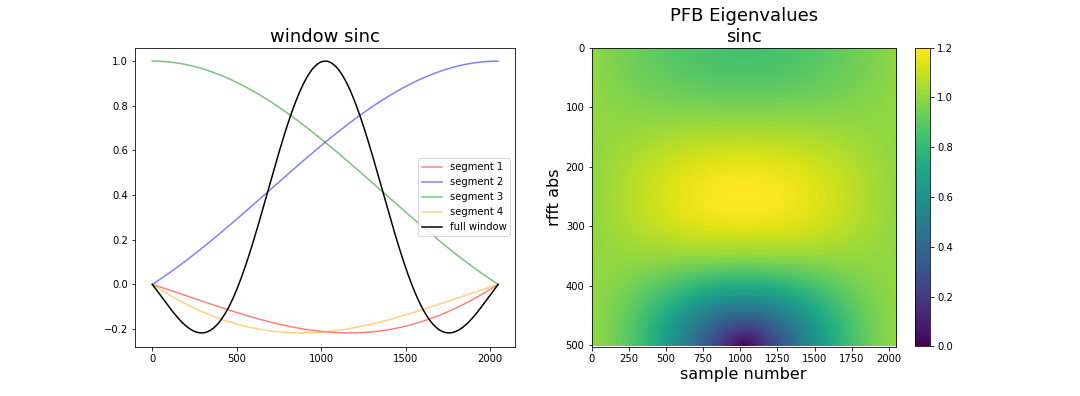
\includegraphics[width=\linewidth]{figures/pfb-colorplot-sinc-window.png}
    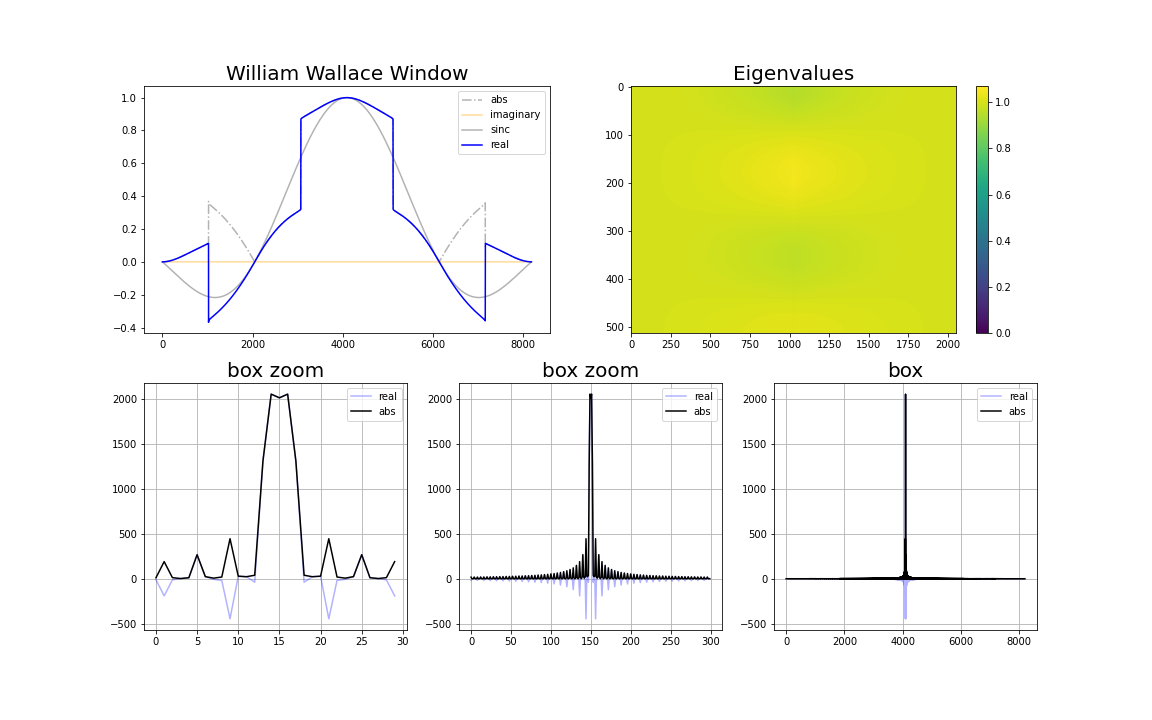
\includegraphics[width=\linewidth]{figures/william_wallace_window_eigenvalues_to_scale.png}
    \caption{Top left is a plot of a window which has a desirable eigenvalue spectrum (right) but a terrible side-lobe problem (bottom).}
    \label{fig:william wallace eigenvalues}
\end{figure}


% \subsection{Inverse matrix method}\label{subsec:}
% 
% \textit{In this section we provide a hand wavy argument that explains how why we think selecting certain eigenvalues will helps us reconstruct the signal. I.e. the thinking that went behind blanking out the eigenvalue.}
% 
% If we know the values of $T-K$ out of the $T$ values $g_n[t]$. Let $S_1$ be the set of $T-K$ known-term times, and let $S_2$ be the set of $K$ unknown-term times. We write our uncertainty in the unknown set of $K$ $g$'s by adding to them a Gaussian random variable 
% 
% $$\lambda[t] \sim \frac{1}{\sqrt{2\pi \sigma_\ast}} \exp\left( -\frac{1}{2} \frac{y^2}{\sigma_\ast^2} \right) \qquad \text{norm dist in }y \qquad t\in S_2$$ 
% 
% where $\sigma_\ast$ comes from \eqref{eq:sigma 0}. \\
% 
% Solving \eqref{eq:coupled equations} for one of the unknown $g[t_0]$ and taking the mean at a particular value of $\xi$ we get. 
% 
% \begin{equation}
% \begin{split}
% \langle g[t_0]\rangle\big|_\xi &= e^{2\pi it_0\xi/T} \left\langle \sqrt T\frac{H_n[\xi] + \hat x[\xi]}{W_n[\xi]} - \sum_{t\in S_1} g[t]e^{-2\pi i t\xi/T} - \sum_{t\in S_2\backslash \{t_0\}}( g[t] + \lambda[t] )e^{-2\pi it\xi/T}\right\rangle \\
% &= e^{2\pi i t_0 \xi/T}\left(\sqrt T  \frac{H_n[\xi]}{W_n[\xi]} - \sum_{t\neq t_0} g[t]e^{-2\pi it\xi/T} \right)
% \end{split}
% \end{equation}
% 
% Computing the variance we find
% 
% \begin{equation}\label{eq:var coupled equations}
% \begin{split}
%     \langle |g[t_0]|^2\rangle - |\langle g[t_0]\rangle|^2 &= T \frac{\langle |\hat x[\xi]|^2\rangle }{|W_n[\xi]|^2} + \sum_{t\in S_2\backslash \{t_0\}} \langle |\lambda[t]|^2\rangle\\
%     &= T\frac{\langle |\hat x[\xi]|^2\rangle}{|W_n[\xi]|^2} + (K-1)\sigma_\ast^2
% \end{split}
% \end{equation}
% 
% Result from scratch work
% 
% $$\sigma_{\text{opt}} \rightarrow \sigma_\ast \sqrt{\frac{K}{T}}$$


\subsection{Inverting the PFB for different values of $\ntap$}\label{sec:eigenvalues different ntaps}

\begin{figure}[H]
    \centering
    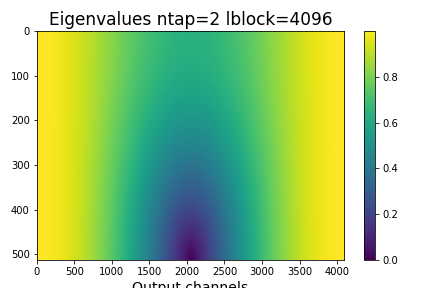
\includegraphics[width=0.4\linewidth]{figures/eigenvalues_ntap/eigenvalues_ntap_2_lblock_4096.png}
    % 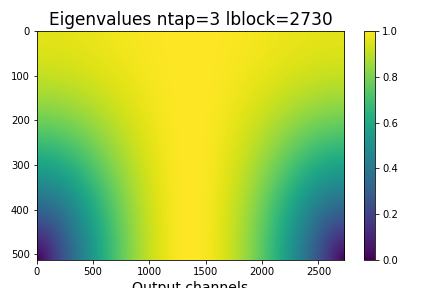
\includegraphics[width=0.3\linewidth]{figures/eigenvalues_ntap/eigenvalues_ntap_3_lblock_2730.png}
    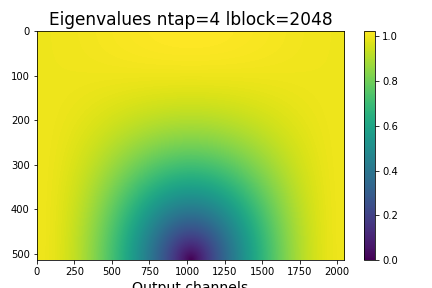
\includegraphics[width=0.4\linewidth]{figures/eigenvalues_ntap/eigenvalues_ntap_4_lblock_2048.png}
    % 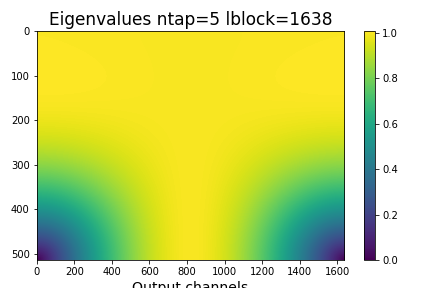
\includegraphics[width=0.3\linewidth]{figures/eigenvalues_ntap/eigenvalues_ntap_5_lblock_1638.png}
    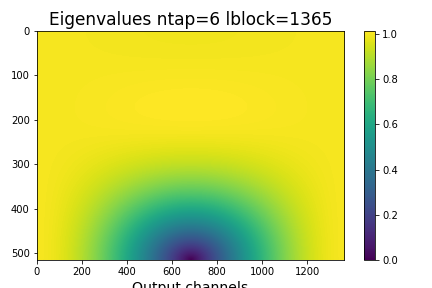
\includegraphics[width=0.4\linewidth]{figures/eigenvalues_ntap/eigenvalues_ntap_6_lblock_1365.png}
    % 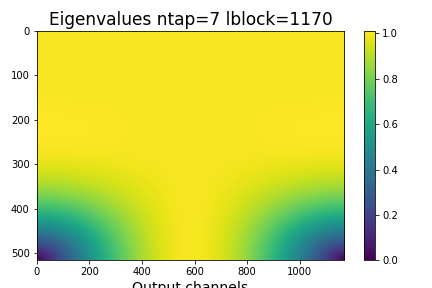
\includegraphics[width=0.3\linewidth]{figures/eigenvalues_ntap/eigenvalues_ntap_7_lblock_1170.png}
    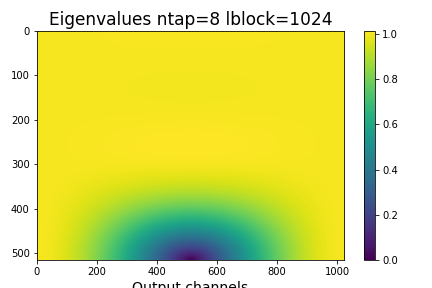
\includegraphics[width=0.4\linewidth]{figures/eigenvalues_ntap/eigenvalues_ntap_8_lblock_1024.png}
    \caption{\textit{Link to the code that generates these plots.} Using less taps makes the signal harder to invert.}
    \label{fig:my_label}
\end{figure}

\end{document}
